\documentclass{article}
                
                
% create a settings file with all settings included                

% package for compiling ASCII input
\usepackage[utf8]{inputenc}
% fontenc – Standard package for selecting font encoding
\usepackage[T1]{fontenc}
% English language package
\usepackage[english]{babel}
% natbib package is used for citations
\usepackage{natbib}
% graphicx – Enhanced support for graphics
\usepackage{graphicx}
% https://ctan.math.illinois.edu/macros/latex/contrib/genealogytree/genealogytree.pdf
\usepackage{genealogytree}
%========================================
% package for hyperlinks
% links also Contents to the appropriate page
\usepackage{hyperref}
\hypersetup{
    colorlinks=true,
    linkcolor=blue,
    filecolor=magenta,      
    urlcolor=cyan,
}
%========================================
% I used this package for the two images task
\usepackage{subfig}
% this package is used to get the different list styles (brackets, roman...)
\usepackage{amssymb}
%prevents figures ever floating backwards up the current page.
\usepackage{flafter}  
% This package provides user control over the layout of the three basic list environments: enumerate, itemize and description.
\usepackage{enumitem} 

%========================================

% TO-DO NOTES

\usepackage{lipsum} % Dummy text
\usepackage{xargs}  % Use more than one optional parameter in a new commands
\usepackage[pdftex,dvipsnames]{}  % Coloured text etc.

% SETUP FOR DIFFERENT TO-DOS SECTIONS
\usepackage[colorinlistoftodos,prependcaption,textsize=tiny]{todonotes}
\newcommandx{\unsure}[2][1=]{\todo[linecolor=red,backgroundcolor=red!25,bordercolor=red,#1]{#2}}
\newcommandx{\change}[2][1=]{\todo[linecolor=blue,backgroundcolor=blue!25,bordercolor=blue,#1]{#2}}
\newcommandx{\info}[2][1=]{\todo[linecolor=green,backgroundcolor=green!25,bordercolor=green,#1]{#2}}
\newcommandx{\improvement}[2][1=]{\todo[linecolor=orange,backgroundcolor=orange!25,bordercolor=orange,#1]{#2}}
\newcommandx{\thiswillnotshow}[2][1=]{\todo[disable,#1]{#2}}

%========================================

% SETUP JAVA CODE

\usepackage{listings}
\usepackage{color}

\definecolor{dkgreen}{rgb}{0,0.6,0}
\definecolor{gray}{rgb}{0.5,0.5,0.5}
\definecolor{mauve}{rgb}{0.58,0,0.82}

\lstset{frame=tb,
  language=Java,
  aboveskip=3mm,
  belowskip=3mm,
  showstringspaces=false,
  columns=flexible,
  basicstyle={\small\ttfamily},
  numbers=none,
  numberstyle=\tiny\color{gray},
  keywordstyle=\color{blue},
  commentstyle=\color{dkgreen},
  stringstyle=\color{mauve},
  breaklines=true,
  breakatwhitespace=true,
  tabsize=3
}
%========================================

\title{Exploration and Presentation \LaTeX}
\author{Jörg Oertel}
\date{March 2021}

\begin{document}

% deletes the front-page page number 
\clearpage\maketitle
\thispagestyle{empty}

\tableofcontents

\clearpage

\section{Introduction}

The first assignment is to find the requirements of a bachelor thesis. The requirements has to be written in \LaTeX and the sources has to be documented.
\linebreak
The second assignment is to produce a template in \LaTeX, that we can use in our bachelor thesis.

\clearpage

\section{Assignment 1}
\begin{enumerate}
    \item Title page without page number
    \item Writing a comment
    \item Table of contents
    \item Danish characters, æ ø å
    \item Graphics
    \begin{itemize}
        \item Image caption
        \begin{itemize}
            \item Caption over Image
            \item Caption under Image
        \end{itemize}
        \item Label
        \item Centering
        \item Two images next to each other
    \end{itemize}
    \item Reference to image
    \item Reference to page containing the image
    \item Section, subsection, paragraph, subparagraph
        \begin{itemize}
            \item Numbered Section
            \item Non-numbered Section
        \end{itemize}
    \item Lists
        \begin{itemize}
            \item Bullet points
            \item Alternative bullet points
            \item Enumerated lists
                \begin{itemize}
                    \item Alternatively numbered lists (roman numerals, letters)
                \end{itemize}
        \end{itemize}
    \item Table with multiple columns
        \begin{itemize}
            \item Various horizontal alignments in columns (left, right, centered)
            \item Cell spanning multiple columns
            \item Vertical alignment in multi-line cells
            \item Table description and label
            \item Reference to table
        \end{itemize}
    \item Code listing
        \begin{itemize}
            \item With emphasized key words in your favorite programming language
        \end{itemize}
    \item Math equations
        \begin{itemize}
            \item Inline equations (in text)
            \item Display equations (on separate line)
            \item Fractions, summations, products, roots, powers
        \end{itemize}
    \item Bibliography with book, article and internet link
    \item To-do notes of own choice
\end{enumerate}



\clearpage
\subsection{Text}

\subsubsection{Title page without page number}

\begin{verbatim}
\clearpage\maketitle
\thispagestyle{empty}
\end{verbatim}

\subsubsection{Writing a comment}
\begin{figure}[h!]
\centering
\includegraphics[scale=0.4]{images/latex_comments.png}
\caption{\LaTeX comments}
\label{fig:comments}
\end{figure}

\subsubsection{Table of contents}
\begin{verbatim}
\tableofcontents
\end{verbatim}

\subsubsection{Danish characters}
\begin{verbatim}
\AA, \aa
\AE, \ae
\O, \o
\end{verbatim}
\AA, \aa \\*
\AE, \ae \\*
\O, \o

\clearpage

\subsection{Graphics}

\subsubsection{Caption over image}
\begin{verbatim}
\includegraphics[scale=0.4]{latex_comments.png}
\caption{\LaTeX comments}
\label{fig:f1}
\end{verbatim}

\subsubsection{Caption under image}
\begin{verbatim}
\caption{\LaTeX comments}
\includegraphics[scale=0.4]{latex_comments.png}
\end{verbatim}

\subsubsection{Label}
\begin{verbatim}
\label{fig:comments}
\end{verbatim}

\subsubsection{Centering}
\begin{verbatim}
\centering
\end{verbatim}

\subsubsection{Two images next to each other}

\begin{figure}[h!]
  \centering
  \subfloat[Version 1]{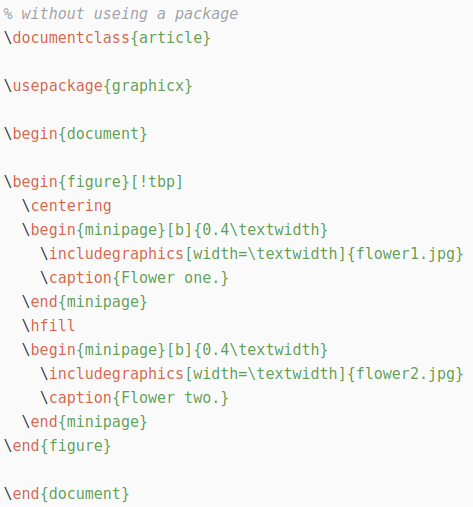
\includegraphics[width=0.4\textwidth]{images/image1.png}\label{fig:f2}}
  \hfill % is used for lining up the images in one row
  \subfloat[Version 2]{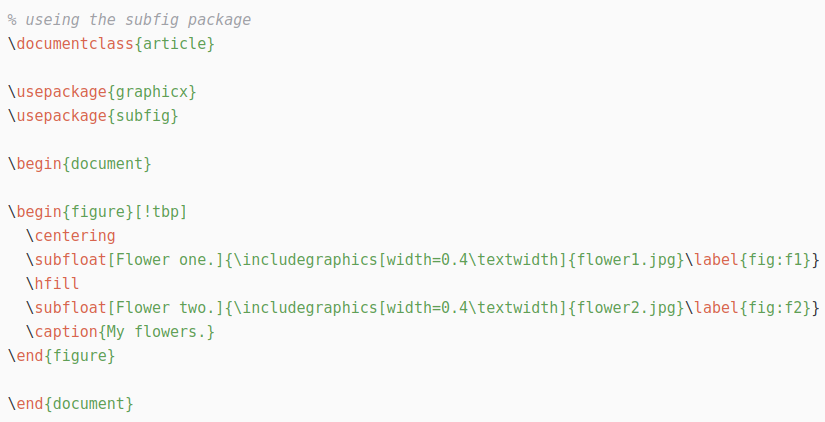
\includegraphics[width=0.4\textwidth]{images/image2.png}\label{fig:f3}}
  \caption{Images}
  \citep{stackexchange}
\end{figure}

\subsubsection{Reference to image}
\begin{verbatim}
\citep{here comes the name of the reference in the bib file}
Reference is shown at the last page.
\end{verbatim}

\subsubsection{Reference to page containing the image}
\begin{verbatim}
see figure \ref{fig:f2} on page \pageref{fig:f2}
\end{verbatim}

\clearpage

\subsection{Lists and Sections}

\subsubsection{Numbered Section}
\begin{verbatim}
\section{First Section}
\section{Second Section}
\end{verbatim}


\subsubsection{Non-Numbered Section}
\begin{verbatim}
\section*{First Section}
\section*{Second Section}
\end{verbatim}

\subsubsection{Bullet points}
\begin{verbatim}
\begin{itemize}
    \item Milk
    \item Sugar
\end{itemize}
\end{verbatim}

\subsubsection{Alternative bullet symbols}
\begin{verbatim}
\renewcommand{\labelitemi}{$\blacksquare$}
\renewcommand\labelitemii{$\square$}
\begin{itemize}
  \item  Milk
  \item  Sugar
\end{itemize}
\end{verbatim}

\subsubsection{Enumerated lists}
\begin{verbatim}
\begin{enumerate}
    \item Milk
    \item Sugar
\end{enumerate}
\end{verbatim}

\subsubsection{Roman numerals, letters}
\paragraph{Roman numbers in enumerate list}
\begin{verbatim}
\begin{enumerate}[label=(\Roman*)]
  \item  Milk
  \item  Sugar
\end{enumerate}
\end{verbatim}

\paragraph{Letters in enumerate list}
\begin{verbatim}
\begin{enumerate}[label=(\roman*)]
  \item  Milk
  \item  Sugar
\end{enumerate}
\end{verbatim}

\subsection{Table with multiple columns}

\subsubsection{Various horizontal alignments in columns (left, right, centered)}

\begin{table}[htp]
    \centering
\begin{tabular}{ | l | c | r | }
\hline
  Left & Center & Right \\ \hline
  Left and Left & Center and Center & Right and Right \\ \hline
  Left & Center & Right \\
\hline
\end{tabular}
    \caption{Caption}
    \label{tab:my_label_1}
\end{table}



\subsubsection{Cell spanning multiple columns}
\begin{table}[htp]
    \centering
    \begin{tabular}{|r|l|}
    \hline
     7C0 & hexadecimal \\
     3700 & octal \\ \cline{2-2}
     11111000000 & binary \\
     \hline \hline
     1984 & decimal \\
    \hline
    \end{tabular}
    \caption{Caption}
    \label{tab:my_label_2}
\end{table}

\subsubsection{Vertical alignment in multi-line cells}


\begin{table}[htp]
    \centering
\begin{tabular}{ |l|l| }
  \hline
  \multicolumn{2}{|c|}{Team sheet} \\
  \hline
  GK & Paul Robinson \\
  LB & Lucas Radebe \\
  DC & Michael Duberry \\
  DC & Dominic Matteo \\
  RB & Dider Domi \\
  MC & David Batty \\
  MC & Eirik Bakke \\
  MC & Jody Morris \\
  FW & Jamie McMaster \\
  ST & Alan Smith \\
  ST & Mark Viduka \\
  \hline
\end{tabular}
    \caption{Caption}
    \label{tab:my_label_3}
\end{table}


\subsubsection{Table description and label}
\begin{verbatim}
    \caption{Description}
    \label{tab:my_label_3}
\end{verbatim}

\subsubsection{Reference to table}
Table~\ref{tab:my_label_1} summarizes Text
\newline
Table~\ref{tab:my_label_2} summarizes Text
\newline
Table~\ref{tab:my_label_3} summarizes Text
\newline
\begin{verbatim}
    Table~\ref{tab:my_label_1} summarizes Text \\
    Table~\ref{tab:my_label_2} summarizes Text \\
    Table~\ref{tab:my_label_3} summarizes Text \\
\end{verbatim}


\subsection{Code listing}

\subsubsection{With emphasized key words in your favorite programming language}

\begin{lstlisting}
// Hello.java
import javax.swing.JApplet;
import java.awt.Graphics;

public class Hello extends JApplet {
    public void paintComponent(Graphics g) {
        g.drawString("Hello, world!", 65, 95);
    }    
}
\end{lstlisting}

\subsection{Math equations}

\subsubsection{Inline equations (in text)}

The well known Pythagorean theorem \(x^2 + y^2 = z^2\) was 
proved to be invalid for other exponents.

\subsubsection{Display equations (on separate line)}

This is a simple math expression
\[\sqrt{x^2+1}\] 
separated from text.

\subsubsection{Numbered equation}
\begin{equation}
E=m
\end{equation}

\subsubsection{Fractions, summations, products, roots, powers}

\begin{enumerate}
    \item \(\frac{1}{2}\)
    \item \(x + y = z\)
    \item \(x * y = z\)
    \item \(\sqrt{x^2+1}\) 
    \item \begin{math}{x^2}\end{math}
    \item \({x^3}\)
\end{enumerate}

\subsection{Bibliography with book, article and internet link}
\subsubsection{Hyperlinks}
\href{http://www.sharelatex.com}{Something Linky}
\begin{verbatim}
\href{http://www.sharelatex.com}{Something Linky}
\end{verbatim}
    
\subsubsection{Bibliography and article}
Bibliographic references are usually kept in a bibliography file whose extension is .bib, this file consists of a list of records and fields. Each bibliography record holds relevant information for a single entry. 


\begin{verbatim}
@article{einstein,
    author =       "Albert Einstein",
    title =        "{Zur Elektrodynamik bewegter K{\"o}rper}. ({German})
        [{On} the electrodynamics of moving bodies]",
    journal =      "Annalen der Physik",
    volume =       "322",
    number =       "10",
    pages =        "891--921",
    year =         "1905",
    DOI =          "http://dx.doi.org/10.1002/andp.19053221004"
}
\end{verbatim}

\subsection{To-do notes of own choice}

\paragraph{see the bottom of the page for the TO-DO note list}

\todo[inline]{The original to-do note without changed colours.\newline Here's another line.}
\lipsum[11]\unsure{Is this correct?}\unsure{I'm unsure about also!}
\lipsum[11]\change{Change this!}
\lipsum[11]\info{This can help me in chapter seven!}
\lipsum[11]\improvement{This really needs to be improved!\newline\newline What was I thinking?!}
\lipsum[11]
\thiswillnotshow{This is hidden since option `disable' is chosen!}
\improvement[inline]{The following section needs to be rewritten!}
\lipsum[11]
\newpage

\clearpage

\section{Assignment 2}
\subsection{Bachelor project}

This document describes the requirements and expectations of your bachelor project.

\subsection{Curriculum}
The curriculum lists the official requirements and learning goals for the bachelor project, as given by Cphbusiness.  
\newline
The requirements, video guide and the examination regulation can be found here:


\begin{itemize}
    \item[] \href{https://www.cphbusiness.dk/media/78341/pbasoftcbastudieordning2017.pdf}{Bachelor requirements}
    \item[] \href{https://www.cphbusiness.dk/media/81380/examination-regulations-cphbusiness-2021.pdf}{Examination Regulations}
    \item[] \href{https://cphbusiness.cloud.panopto.eu/Panopto/Pages/Viewer.aspx?id=38f9e1bf-333f-44d7-a47b-a85e00bcbc5d&query=data20science}{Structure of bachelor project}
    \item[] \href{https://cphbusiness.cloud.panopto.eu/Panopto/Pages/Viewer.aspx?id=7899543a-eddd-49b9-9ffc-a85e00c1a56e&query=data20science}{Evaluation Criteria for the Bachelor Project}
\end{itemize}

\subsection{The project}
The bachelor project is a project where the student investigates a software-related problem, propose a solution, and does some implementation to demonstrate the solution. The student should strive to  include elements from the courses passed during the program (Large Systems Development, Databases Testing, System Integration).The project may be done in groups of up to 4 people. Having a larger group should increase the project scope, as it raises the general expectations of the project. The project covers 15 EC-TS points, which is roughly equivalent to 
\begin{center}15·27.4 hours = 412.5 hours\end{center}

\subsection{Report}
\textbf{Size of Report:} The maximum page count for the bachelor report is given by the formula below.
\begin{center}maxPageCount = 40 + 20·numberOfStudents\end{center}
Reports shorter than \(\frac{2}{3}\) will usually be experienced as short, although there is no official minimum size.
\newline
\newline
\textbf{Language:} The report can be written in either Danish or English.
\newline
\newline
\textbf{Contents:} The report should contain a thorough description of the work that has been done during the bachelor project, as well as an evaluation and reflection on the work.

\subsection{Report components}
The instructors recommend the following sections to be in the report. The components of the report do not have to be presented in exactly the same order but are recommended to be present.

\subsubsection{Project title}
\textbf{Cover page:} Project title, your name and student identification, school and supervisor.
\newline
\subsubsection{Abstract}
\textbf{Four sentences:} Problem statement, further elaborated  in  Introduction. It can be seen as an advertisement for the rest of the report. The final abstract is written in the end of the project.

\begin{itemize}
    \item What is the problem ?
    \item Why is the problem interesting ?
    \item What is the solution
    \item What are the implementation ?
\end{itemize}

\subsection{Introduction}

\textbf{Project summary:}
\begin{itemize}
    \item Motivation - Why this topic is important nowadays.
    \item Project objectives — what is the expected result.
    \item Project tasks — what is to be done for achievement of the objectives-steps in the work, such as getting acquainted with the state-of-the-art and trends in the area, selecting a development methodology, creating a design, selecting development tools and environments, programming, testing,  implementation and evaluation, as appropriate.
    \item Scope of the project — what is not an objective or a task.
    \item Brief description of the other chapters that follow — one paragraph per each.
\end{itemize}

\subsubsection{State of the art and trends}
Survey of current technologies and similar solutions in this area – to show that you are well informed and step on the available achievements: For example, you can present some relevant knowledge gathered from both previously studied modules and external sources, organized in a structured form. Here you can also describe and compare alternative development methodologies, technologies, environments, frameworks, or programming languages that could have been used, and to explain and argue your choice. Inside the text, a citation or a reference to the used sources (books, articles, web pages) is required. The sources can be listed either underscore, or in an Appendix.

\subsubsection{Requirements specification and solution design}
Formulation of project foundation – a solid ground of your solution: This part reflects the design process, or the methodology you have followed. Analysis – who are the users, use-cases and scenarios,  intended user experiences. The analysis lead to specifications – formal functional and non-functional requirement to the application. Specifications lead to requirements: you consider how to design the  solution– system architecture, data models, visual interface, control, operability, algorithms,  integration and other components, as appropriate. Use graphics for visual presentation of your concepts as much as possible.

\subsubsection{Solution development and implementation}
Presentation of the application, test procedures, deployment and maintenance environments: This  part presents the product in technical terms. Implementation and test environment— test strategies, test plan, test suites, demo and screen captures, usability evaluation, etc. Units of code, packages, deployment, supported interfaces, algorithms, input and output, supported file formats, frameworks,  servers and clients, etc.

\subsubsection{Conclusions}
Brief summary: What has been done and the benefits of it. Recommendation for future extensions and upgrades. Reflection on the work and the product.

\subsubsection{Appendices}
Reference of information sources as many, as possible, listed according a standard - see:
\newline
\href{https://ieee-dataport.org/sites/default/files/analysis/27/IEEE20Citation20Guidelines.pdf)}{Reference standard}   
\newline
Installation guide and/or user manual, if appropriate. Source code of main components, if appropriate.

\subsubsection{Final  works}
Project and documentation completed. Visual (power  point) presentation and a demo prepared. It is recommended to discuss the draft-report with the supervisor before the final!

\clearpage

\section{Conclusion}
``I always thought something was fundamentally wrong with the universe'' \citep{adams1995hitchhiker}


\clearpage

\bibliographystyle{plain}
\bibliography{bib/references}
\listoftodos[Notes]
\end{document}
